\documentclass{article}
\usepackage[utf8]{inputenc}
\usepackage{amsmath}
\usepackage{fullpage}
\usepackage{graphicx}
\usepackage{url}

\title{Solar heating simulation}
\author{Mohit Tekriwal}
\date{}



\begin{document}

\maketitle

In this assignment, we are asked to simulate the heat transfer from a solar panel to a storage tank. 

\subsubsection*{Assumptions in the system}
We will assume the following throughout the simulation:

\begin{enumerate}
\item The mass flow rate through the flow loop is constant
\item The specific heat capacity of water is constant through out the loop. This assumption is sound because the temperature fluctuation of water in the loop is not high.
\item We will assume laminar flow in the pipe, and therefore the convective heat transfer coefficient will correspond to that of the laminar region. Also the convection is forced.
\item To capture the temperature gradient in the storage tank, we will divide the tank into uniform blocks, and each of these blocks have the same convective heat transfer coefficient.
\item There is no heat loss in the pipe.

\end{enumerate}

\subsubsection*{Modeling flow in the storage tank}
We will model the storage tanks using  $N$ uniform blocks. Each of these blocks therefore has the same area. The upper most block which receives water from the collector will be called as \emph{Node $0$}, while the bottom most block which is connected to the inlet of the collector will be called as \emph{Node $N-1$}.The flow of water is from node $0$ to node $N-1$.  The figure~\ref{fig: heat_tank} illustrates the heat flow inside the stratified tank. The heat transfer equation for each of these block in as illustrated in the figure, is given by [1]:

\begin{equation}
mC_p \frac{dT_{s, i}}{dt} = U_i A_i (T_a - T_{s,i}) + B_c^i \dot{m} C_p (T_c - T_{s,i}) + \gamma_i C_p (T_{s, i-1} - T_{s,i})
\end{equation}
where $C_p$ is the specific heat capacity of water,$T_c$ is the temperature of the water coming out of the collector, $T_a$ is the ambient temperature, $T_{s, i}$ is the temperature of the $i-th$ block in the storage tank.  $U_i$ is the heat loss coefficient for each node. Overall tank heat loss coefficient is assumed to be 2.5 $KJ/h m^2 K$ . $A_i$ is the area for each node.
$B_c^i$ is a collector control function, which can be defined to identify which node receives water from the collectors, and is given by the following formula:
\begin{equation}
B_c^i = 
\begin{cases}
 1 \quad if \quad T_{s_i-1} > T_c > T_{s,i} \\
 0 \quad other  
\end{cases}
\end{equation}

$\gamma_i$ is the net flow between the nodes, and is given by the formula [1]:
\begin{equation}
\gamma_i = \dot{m} \sum_{j = 1} ^{i-1} B_c^j
\end{equation}
The above modeling is generic, where generalization is in terms of the placement of the inlet from the collector into the tank. For this particular problem, $B_c^i = 1$ only for node $0$, and is $0$ for all other nodes, since the inlet of the tank is fixed on the upper layer.

\begin{figure}[ht]
\centering
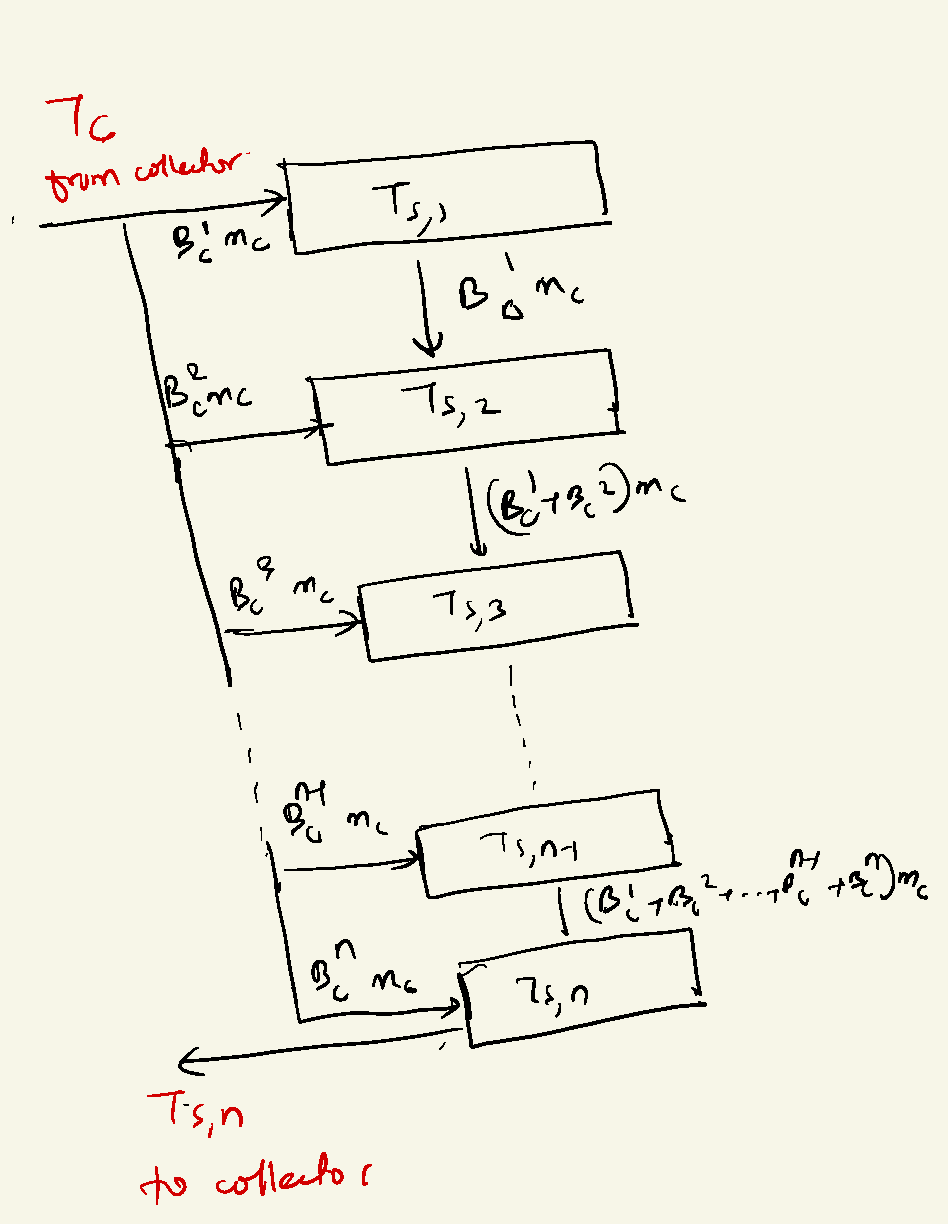
\includegraphics[scale = 0.5]{Diagram.pdf}
\caption{Figure illustrating the heat transfer inside the stratified storage tank.}
\label{fig: heat_tank}
\end{figure}






\subsubsection*{Heat balance for the collector}
The useful energy gain, $\dot{Q}_u$ for a flat-plate collector can be computed using the Hottel- Whillier equation [1]:
\begin{equation}
\dot{Q}_u = A_c [F_R (\tau \alpha) I_T- F_R U_L (T_{in} - T_a)] =  \dot{m} C_p (T_c - T_{in})
\end{equation}
where $A_c$ is the total collector area, $F_R$ is the collector heat removal factor, $\tau \alpha$ is the transmittance- absorptance product, and $U_L$ is the overall loss coefficient between the collector and the environment per unit area. To optimize the system, characteristic factors from the standard test data (Fanney and Klein, 1983) have been selected:
$F_R (\tau \alpha) = 0.84$ and $F_R U_L = 1.89 W / s m^2 \deg  C$. $I_T$ is the solar radiation incident rate on the collector per unit area, $W /m^2$. As a reference point, a daily sinusoidal radiation profile between hour 7 and 17 of the day with a total irradiance of 13.5 $MJ . (m^2 day)$ or 93.73 $W/m^2$ is used.
Hence, the temperature of water coming out of the collector is given by the formula:
\begin{equation}\label{collector_temp}
T_c = T_{in} + A_c \frac{F_R (\tau \alpha)  I_T - F_R U_L (T_{in} - T_a)} { \dot{m} C_p}
\end{equation}


\subsubsection*{Numerical solution to the heat balance equation for storage tank and the collector}
In this work, I will be discretizing the first order derivative $\frac {dT_{s,i}} {dt} $ using the Euler formula for forward error finite difference scheme. Therefore denoting,
\begin{equation*}
R_i^n := U_i A_i (T_a - T_{s,i}) + B_c^i \dot{m} C_p (T_c - T_{s,i}) + \gamma_i C_p (T_{s, i-1} - T_{s,i})
\end{equation*}
we get the temperature at the next marching step by
\begin{equation}
m C_p \frac {T_{s,i}^{n+1} - T_{s,i}^n} {\Delta t} = R_i^n \implies T_{s,i}^{n+1} =  T_{s,i}^n + (R_i^n \Delta t) / (m C_p)
\end{equation}
where $\Delta t = t / N$, is the uniform time step size, and $N$ is a parameter which describes the number of time steps to be taken from initial time step to a user specified time horizon $t$. I assign the initial temperature profile for the blocks of storage tank to be the ambient temperature, $T_a$.  For any given time step, the inlet temperature or temperature of node $0$, $T_{s, o} = T_C$ is the collector temperature. The outlet temperature of the storage tank or the inlet temperature for the collector, $T_{in} = T_{s, N-1}$. The collector temperature, $T_c$ at any time step is given by~(\ref{collector_temp}).


\subsubsection*{Overview of the code}
The main file which implements the physics of heat transfer is called \texttt{simulation.cpp}. The module \texttt{collector\_temp} gives the collector temperature:
\begin{verbatim}
// Module for collector
// Input: T_n
// Output: T_c
double collector_temp(double T_N);
\end{verbatim}
The module \texttt{temp\_profile\_storage\_tank} returns the instantaneous temperature profile in the tank.
\begin{verbatim}
// Module for computing the temperature profile in a tank
// Input : Initial temperature profile
// Output: Instantaneous temperature profile
vector<double> temp_profile_storage_tank(vector<double> &init_temp_profile, double time);
\end{verbatim}
As discussed above, the initial temperature profile of the storage tank before beginning the simulation is assigned to $T_a$.
\begin{verbatim}
 // intitial temperature profile
    vector<double> init_temp_profile;
    for (int i = 0; i < n; i++)
        init_temp_profile.push_back(T_a);
\end{verbatim}
To run the simulation just run the script file \texttt{run.sh}. To generate a plot illustrating the temperature profile in the storage tank, run the script file \texttt{plot.sh}. The plotting is done using GNUPlot.


\subsubsection*{Results}
With the following inputs defined in the \texttt{global\_variables.h} header file:
\begin{verbatim}
int n = 10; // Number of layers in a tank
int no_of_time_steps = 100;
double I_solar = 93.75; // Solar radiation rate: W/m^2
double F_r_t_alpha = 0.84; 
double F_r_U_L  = 1.89; // W / s m^2 C
double m_dot = 0.1; // Mass flow rate: Kg / s
double T_a = 25.0; // Ambient temperature
double Cp = 1.1630555555556 ; // Specific heat coefficient og water: W / Kg / C
double U = 0.694;
//double U = 0.0;
double H = 1; // Height of tank  = 1m
double d = 0.5; // Diameter of tank = 0.5m
double A = 2 * 3.14 * (d/2) * (H /n); // Surface area of water
double A_c = 0.0419354; // in m^2 Typical dimension: 65 inches by 39 inches
double m_s = 0.997 * (3.14 * (d/2) * (d/2)* (H * 1./n)); // mass of water in a layer of tank
\end{verbatim}
The collector outlet temperature is computed as 53.4179 Celsius, and the collector inlet temperature is computed as  25.0741 Celsius.

\begin{figure}[ht]
\centering
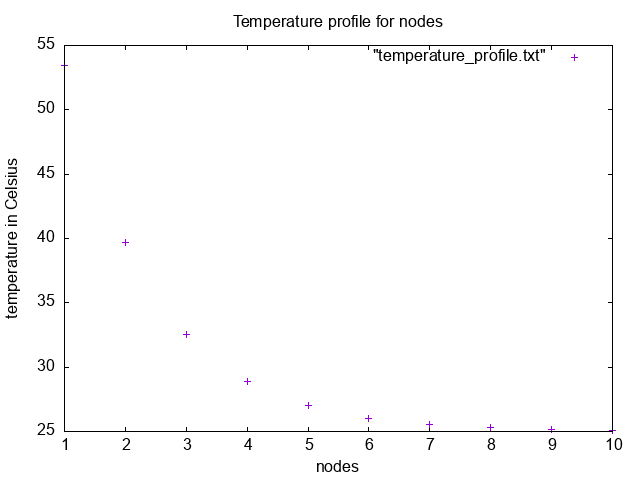
\includegraphics[scale = 0.5]{figures/temperature_profile.png}
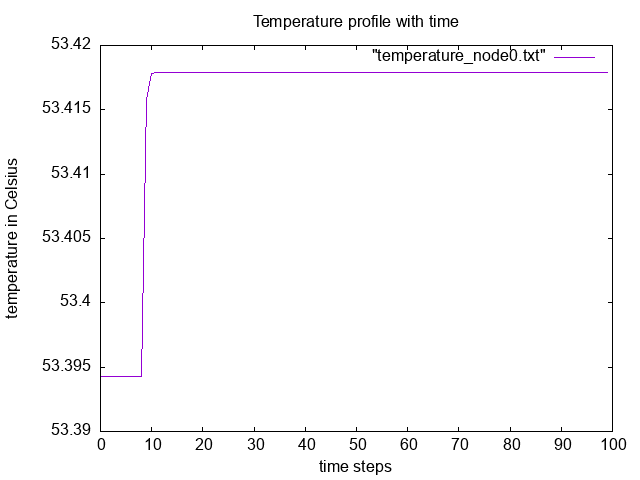
\includegraphics[scale =0.5]{figures/temperature_node0.png}
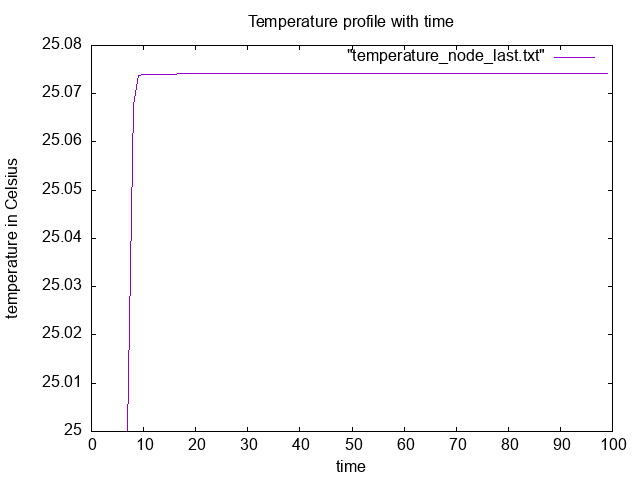
\includegraphics[scale =0.5]{figures/temperature_node_last.png}
\caption{Plot for temperature profiles corresponding to the discretization of the storage tank by 10 nodes. The first figure illustrates the temperature profile along the tank from top to bottom. The second figure illustrates the variation of temperature for Node 0 with respect to time, and the last figure illustrates the variation of temperature for the last node with respect time. Note that this model accounts for the loss of heat to the surrounding, hence $U \neq 0$}.
\end{figure}

\begin{figure}[ht]
\centering
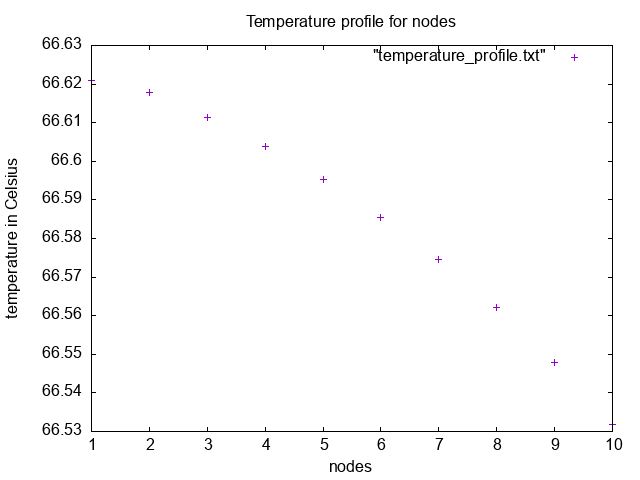
\includegraphics[scale = 0.5]{figures/temperature_profile_u_0.png}
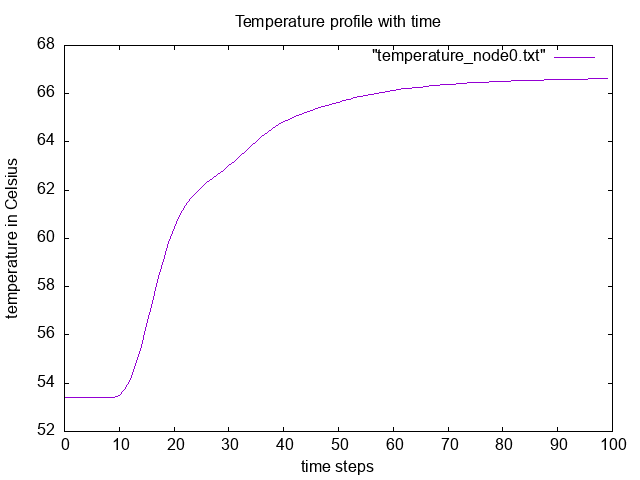
\includegraphics[scale =0.5]{figures/temperature_node0_u_0.png}
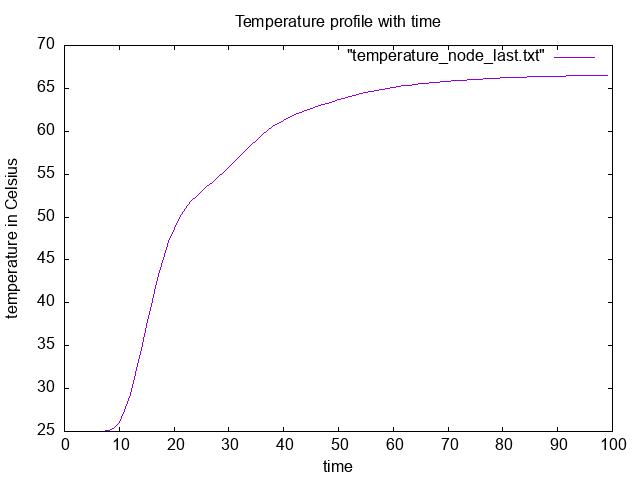
\includegraphics[scale =0.5]{figures/temperature_node_last_u_0.png}
\caption{Plot for temperature profiles corresponding to the discretization of the storage tank by 10 nodes. The first figure illustrates the temperature profile along the tank from top to bottom. The second figure illustrates the variation of temperature for Node 0 with respect to time, and the last figure illustrates the variation of temperature for the last node with respect time. Note that this model does not account for the loss of heat to the surrounding, hence $U =  0$}.
\end{figure}

\begin{figure}[ht]
\centering
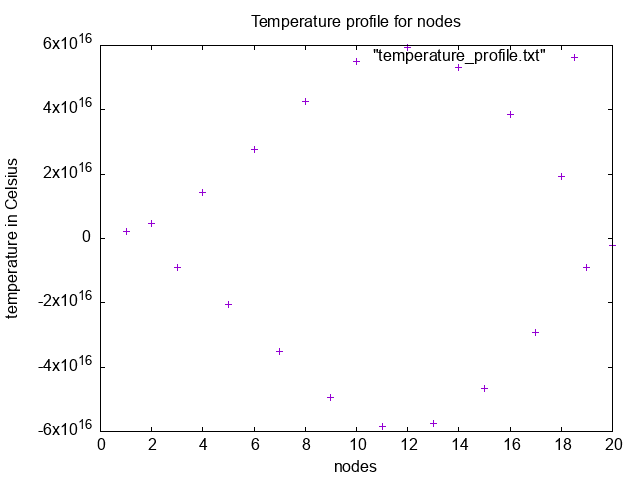
\includegraphics[scale = 0.5]{figures/temperature_profile_N_20_dt_100.png}
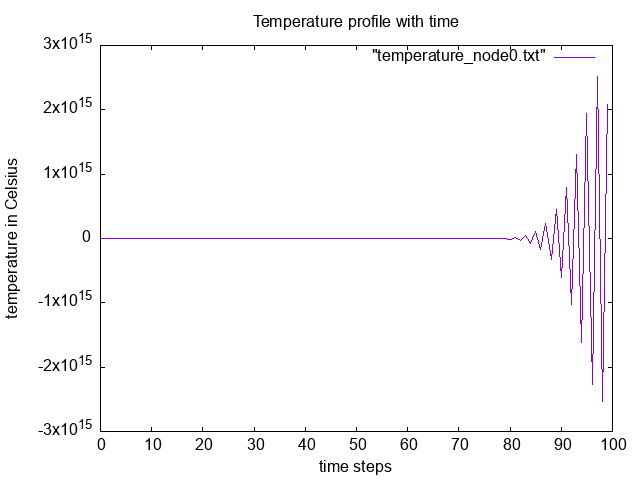
\includegraphics[scale =0.5]{figures/temperature_node0_N_20_dt_100.png}
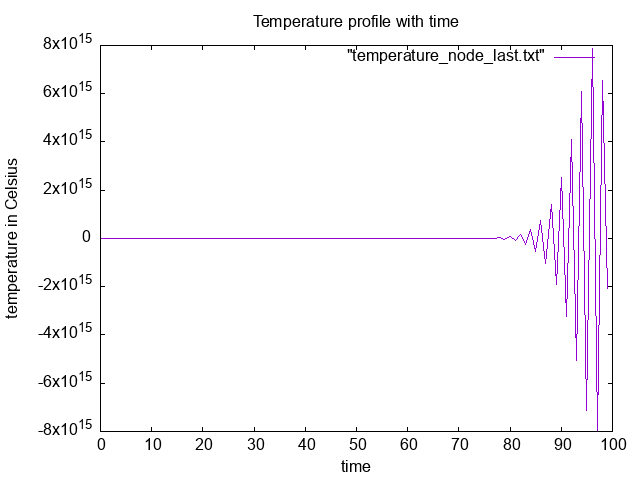
\includegraphics[scale =0.5]{figures/temperature_node_last_N_20_dt_100.png}
\caption{Plot for temperature profiles corresponding to the discretization of the storage tank by 20 nodes. The first figure illustrates the temperature profile along the tank from top to bottom. The second figure illustrates the variation of temperature for Node 0 with respect to time, and the last figure illustrates the variation of temperature for the last node with respect time. Note that this model accounts for the loss of heat to the surrounding, hence $U \neq 0$. Number of time steps is 100. We get numerical instabilities.}
\end{figure}

\begin{figure}[ht]
\centering
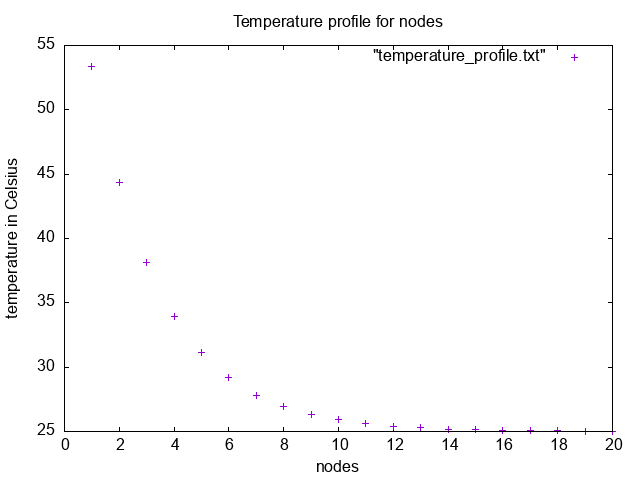
\includegraphics[scale = 0.5]{figures/temperature_profile_N_20.png}
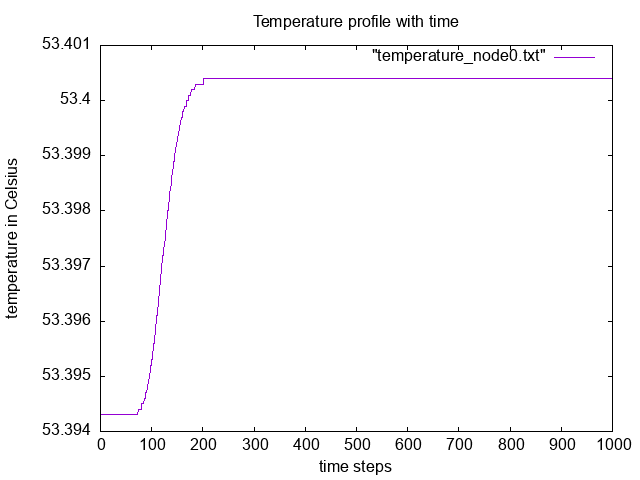
\includegraphics[scale =0.5]{figures/temperature_node0_N_20.png}
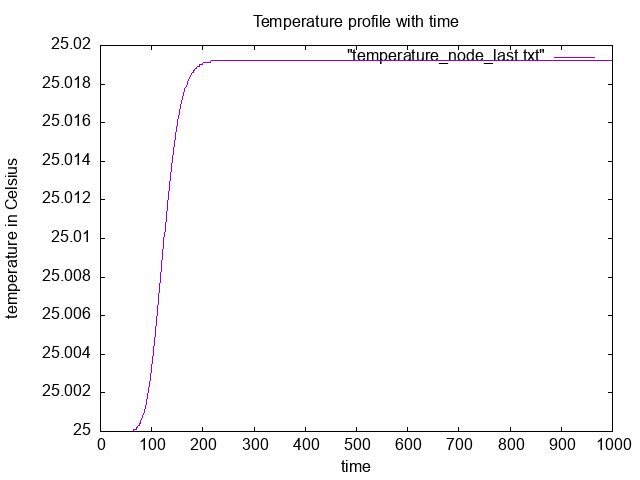
\includegraphics[scale =0.5]{figures/temperature_node_last_N_20.png}
\caption{Plot for temperature profiles corresponding to the discretization of the storage tank by 20 nodes. The first figure illustrates the temperature profile along the tank from top to bottom. The second figure illustrates the variation of temperature for Node 0 with respect to time, and the last figure illustrates the variation of temperature for the last node with respect time. Note that this model accounts for the loss of heat to the surrounding, hence $U \neq 0$. Number of time steps is 1000.}
\end{figure}

\begin{figure}[ht]
\centering
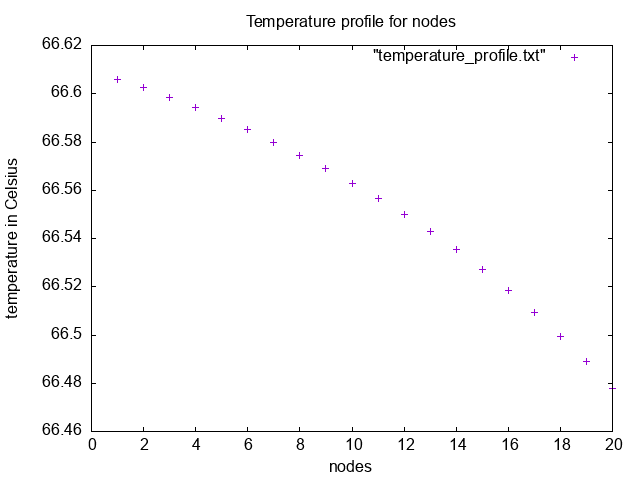
\includegraphics[scale = 0.5]{figures/temperature_profile_N_20_U_0.png}
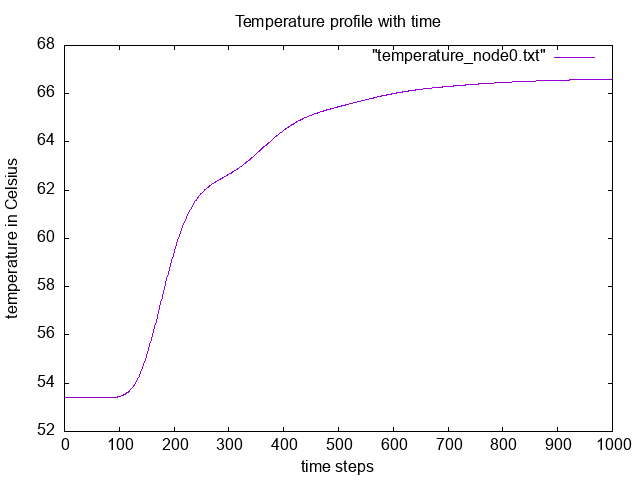
\includegraphics[scale =0.5]{figures/temperature_node0_N_20_U_0.png}
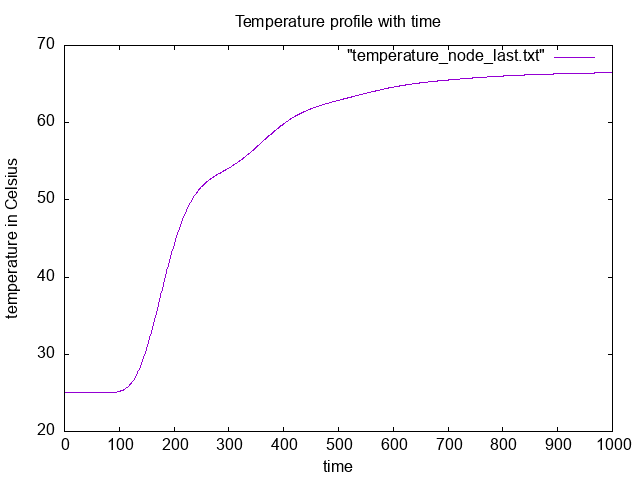
\includegraphics[scale =0.5]{figures/temperature_node_last_N_20_U_0.png}
\caption{Plot for temperature profiles corresponding to the discretization of the storage tank by 20 nodes. The first figure illustrates the temperature profile along the tank from top to bottom. The second figure illustrates the variation of temperature for Node 0 with respect to time, and the last figure illustrates the variation of temperature for the last node with respect time. Note that this model does not account for the loss of heat to the surrounding, hence $U = 0$. Number of time steps is 1000. }
\end{figure}

\begin{figure}[ht]
\centering
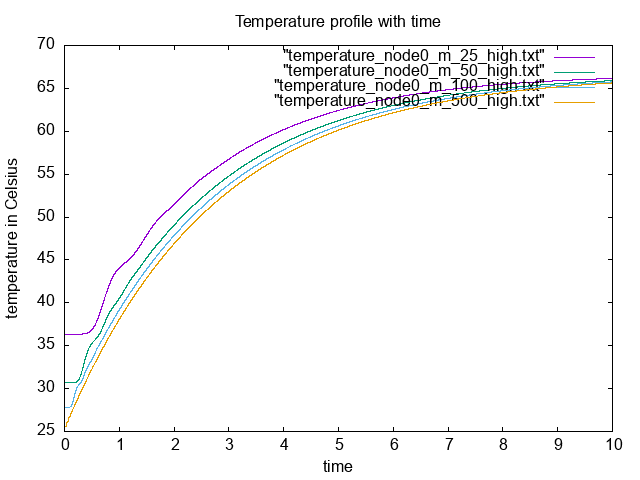
\includegraphics[scale = 0.5]{figures/temperature_node0_mdot.png}
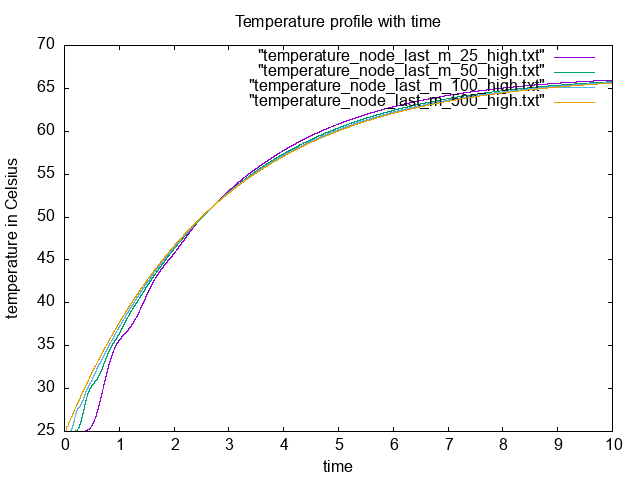
\includegraphics[scale = 0.5]{figures/temperature_node_last_mdot.png}
\caption{Plot for temperature profiles corresponding to the discretization of the storage tank by 20 nodes. Note that this model does not account for the loss of heat to the surrounding, hence $U = 0$. This plot illustrates the effect of mass flow rate on the temperature profile of the nodes in the tank.  Plots are shown for $\dot{m} = 0.25 Kg/s$, $\dot{m} = 0.5 Kg/s$, $\dot{m} = 1.0 Kg/s$, and $\dot{m} = 5.0 Kg/s$ from top to bottom. As observed, time taken for the temperatures in the tank to reach a steady state increases as we increase the mass flow rate.  Thus, for a given time horizon, the circulating water gets heated more and has higher temperature for lower mass flow rate, as compared to the higher mass flow rate. }
\end{figure}

\begin{figure}[ht]
\centering
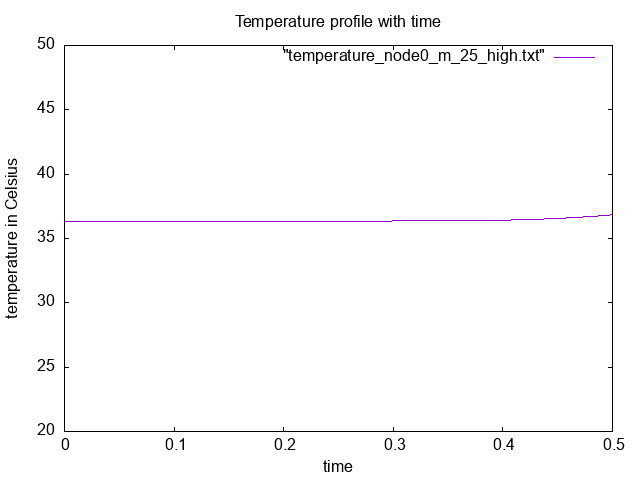
\includegraphics[scale =0.4]{figures/temperature_node0_N_20_m_25.png}
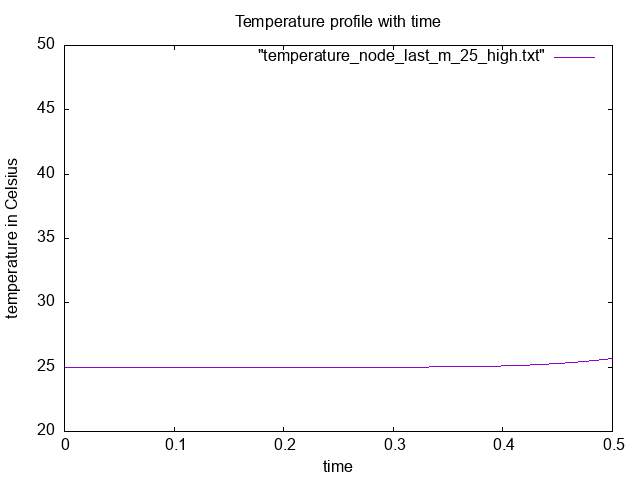
\includegraphics[scale =0.4]{figures/temperature_node_last_N_20_m_25.png}
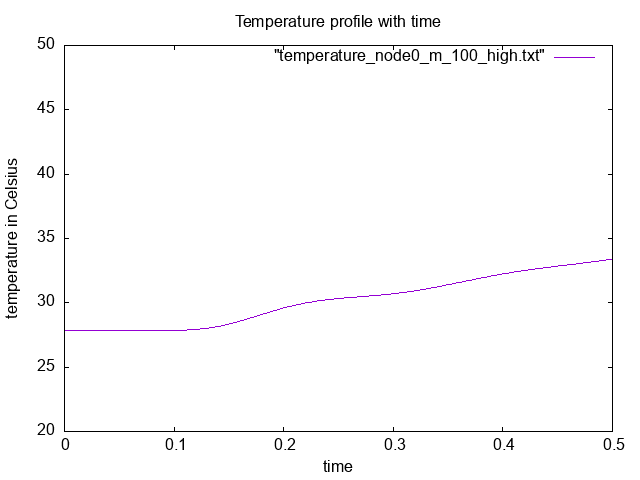
\includegraphics[scale =0.4]{figures/temperature_node0_N_20_m_100.png}
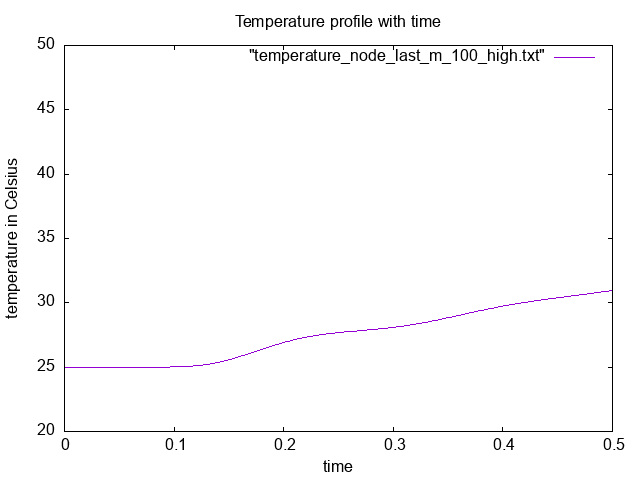
\includegraphics[scale =0.4]{figures/temperature_node_last_N_20_m_100.png}
\caption{Plot for temperature profiles corresponding to the discretization of the storage tank by 20 nodes. Note that this model does not account for the loss of heat to the surrounding, hence $U = 0$. The top left and top right plots correspond to $\dot{m} = 0.25 Kg/s$, while the bottom left and bottom right plots correspond to $\dot{m} = 1.0 Kg/s$. As observed, the time taken for the temperatures in a layer of the tank to remain invariant increases as we increase the mass flow rate. In this example, the time taken for temperature to remain invariant is almost 4 times for $\dot{m} = 0.25 Kg/s$ as compared to $\dot{m} = 1.0 Kg/s$.}
\end{figure}

\begin{figure}[ht]
\centering
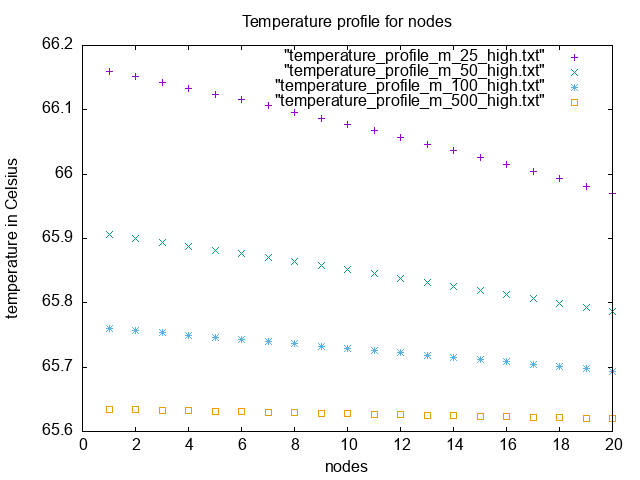
\includegraphics{figures/temperature_profile_m_dot.png}
\caption{Plot for temperature profiles corresponding to the discretization of the storage tank by 20 nodes. Note that this model does not account for the loss of heat to the surrounding, hence $U = 0$. This plot illustrates the effect of mass flow rate on the temperature profile of the nodes in the tank.  Plots are shown for $\dot{m} = 0.25 Kg/s$, $\dot{m} = 0.5 Kg/s$, $\dot{m} = 1.0 Kg/s$, and $\dot{m} = 5.0 Kg/s$ from top to bottom. As observed, time taken for the temperatures in the tank to reach a steady state increases as we increase the mass flow rate.  Thus, for a given time horizon, the circulating water gets heated more and has higher temperature for lower mass flow rate, as compared to the higher mass flow rate. The temperature profile for different mass flow rates eventually converge to a steady state profile.  }
\end{figure}

\newpage
\subsubsection*{Discussion of the results}
In this simulation, I have studied the effect of three parameters, which have been illustrated in the plots.

\begin{enumerate}
\item
\textbf{effect of tank heat loss coefficient:} I have considered two cases - $U \neq 0$ and $U = 0$, i.e., corresponding to the cases when heat is lost to the surrounding and no heat is lost to the surrounding, respectively. As illustrated by the temperature gradient along the tank in Figure 2 and 3, we observe that when $U \neq 0$, temperature decreases along the stratified tank from the top to bottom. On the other hand, when there is no loss of heat to the surrounding, the temperature is almost the same throughout the tank, and the temperature gradient along the tank is low. Also, since there is no loss of heat to the surrounding the effective temperature of water in the tank is higher than when $U \neq 0$, as evident from the higher maximum temperature in the tank for $U = 0$ case.

\item
\textbf{effect of mass flow rate of water:}
In this assignment, I have varied the mass flow rates and studied it for four different mass flow rates: $\dot{m} = 0.25, 0.5, 1.0, 5.0 Kg/s$. As observed in the figure 7, 8 and 9, mass flow rate affects the rate at which water is heated in the tank. Lower the mass flow rate, lower will be the time taken for the water in the tank to be heated, while it takes longer to heat the tank if the mass flow rate is higher. Also, higher the mass flow rate, lower will be the temperature gradient along the tank. This is evident from the slope of the curve in Figure 9. 

\item
\textbf{effect of time step size and spatial discretization along the tank:}
Since we are using an explicit time integration scheme, the numerical stability of the method would depend on the size of time step and discretization along the tank. This is evident from the figures 3, 4 and 5. In figure 3 and 4, I use the same time step even though the spatial discretization is halved in Figure 4 (Figure 3 uses 10 nodes, while Figure 4 uses 20 nodes). We can observe that the numerical solution blows up for $N = 20$ for the same time-step. However, as I decrease the time step by a factor of 10 as in figure 5, the numerical solution does not blow up and the numerical integration is stable. Thus, we need to choose the time step carefully for the method to yield stable numerical solution.

\end{enumerate}
We also observe that at any given node, the temperature increases with time, till it becomes stagnant after a certain period of time, assuming the numerical integration is stable.

We can study the system by tuning other parameters in the \texttt{global\_variables.h} header file. I just limit my study to these three parameters for the sake of brevity. 


\subsubsection*{References}
[1]I mainly followed the masters thesis by Eberhard Markus Kleinbach titled "Performance Study of One-Dimensional Models for Stratified Thermal Storage Tank": \url{https://doi.org/10.1016/0038-092X(93)90087-5}.

\end{document}

